\documentclass{beamer}

% \documentclass[draft]{beamer}
% \includeonlyframes{wip}

% This file is a solution template for:

% - Giving a talk on some subject.
% - The talk is between 15min and 45min long.
% - Style is ornate.



\mode<presentation>
{
  \usetheme{Warsaw}
  % or ...

  \setbeamercovered{transparent}
  % or whatever (possibly just delete it)
}


\usepackage[dutch]{babel}
\usepackage[utf8]{inputenc}
\usepackage{times}
\usepackage[T1]{fontenc}

\usepackage{mathtools}
\usepackage{tikz}

\usetikzlibrary{arrows,external}
\usepackage{pgfplots}
\pgfplotsset{compat=1.10}
\usepackage[detect-family]{siunitx}
\usepackage[eulergreek]{sansmath}
\sisetup{text-sf=\sansmath}
\usepackage{relsize}


\graphicspath{{figures/}}


\title{Statistische data-analyse 1}
\subtitle{Onzekerheden en de normale verdeling}
\author{David Fokkema}
\institute{
  Practicum natuurkunde \\
  Vrije Universiteit / Universiteit van Amsterdam
}
\date{9 januari 2017}

\subject{Colleges}
% This is only inserted into the PDF information catalog. Can be left
% out.



% If you have a file called "university-logo-filename.xxx", where xxx
% is a graphic format that can be processed by latex or pdflatex,
% resp., then you can add a logo as follows:

% \pgfdeclareimage[height=0.5cm]{university-logo}{university-logo-filename}
% \logo{\pgfuseimage{university-logo}}



% Delete this, if you do not want the table of contents to pop up at
% the beginning of each subsection:
\AtBeginSubsection[]
{
  \begin{frame}<beamer>{Outline}
    \tableofcontents[currentsection,currentsubsection]
  \end{frame}
}


% If you wish to uncover everything in a step-wise fashion, uncomment
% the following command:

%\beamerdefaultoverlayspecification{<+->}


\begin{document}

\begin{frame}
  \titlepage
\end{frame}

\begin{frame}{Outline}
  \tableofcontents
  % You might wish to add the option [pausesections]
\end{frame}


% Since this a solution template for a generic talk, very little can
% be said about how it should be structured. However, the talk length
% of between 15min and 45min and the theme suggest that you stick to
% the following rules:

% - Exactly two or three sections (other than the summary).
% - At *most* three subsections per section.
% - Talk about 30s to 2min per frame. So there should be between about
%   15 and 30 frames, all told.

\section{Inleiding}

\begin{frame}{}
\end{frame}


\section{Onzekerheden}

\begin{frame}{Foutenberekening}
  \begin{itemize}
    \item Vorig jaar: foutenberekening
    \item Onzekerheden uit verschillende bronnen combineren tot totale onzekerheid
    \item Voorbeeld:
    \begin{equation*}
        P = \frac{U^2}{R} \qquad
        \visible<1>
        {\mathrlap{\delta P = \ ?}}
        \visible<2>
        {\mathrlap{\delta P = \sqrt{\left(\frac{\partial P}{\partial U}\delta U\right)^2 + \left(\frac{\partial P}{\partial R}\delta R\right)^2}}}
        \visible<3>
        {\frac{\delta P}{P} = \sqrt{\left(2\frac{\delta U}{U}\right)^2 + \left(\frac{\delta R}{R}\right)^2}}
    \end{equation*}
  \end{itemize}
\end{frame}

\begin{frame}{Onzekerheid verkleinen}
  Hoe verklein je de onzekerheid in een experiment?
  \begin{itemize}
    \item nauwkeuriger meten
    \item<2-> \alert{vaker} meten!
  \end{itemize}
\end{frame}

\begin{frame}{Vaker meten (1)}
  \dots geeft een nauwkeurige schatting van de werkelijke waarde $X$
  \begin{center}
    \begin{tikzpicture}
      \draw[thick] (-5, 0) -- (5, 0);
      \path (0, 30pt) -- (0, -30pt);
      \only<2>{\input{scripts/slide-vaakmeten-gemiddelde-1.out}}
      \only<3>{\input{scripts/slide-vaakmeten-gemiddelde-2.out}}
      \only<4>{\input{scripts/slide-vaakmeten-gemiddelde-3.out}}
      \only<5>{\input{scripts/slide-vaakmeten-gemiddelde-4.out}}
      \only<6>{\input{scripts/slide-vaakmeten-gemiddelde-5.out}}
    \end{tikzpicture}
  \end{center}
  \visible<6>
  {Goede schatter is het gemiddelde $\bar x$:
  \begin{equation*}
    \bar x = \frac{1}{N}\sum_{i=1}^{N} x_i.
  \end{equation*}}
\end{frame}

\begin{frame}{Vaker meten (2)}
  \dots geeft een nauwkeurige schatting van de onzekerheid op \alert{individuele} meting
  \begin{center}
    \begin{tikzpicture}
      \draw[thick] (-5, 0) -- (5, 0);
      \path (0, 35pt) -- (0, -35pt);
      \only<2>{\input{scripts/slide-vaakmeten-stddev-1.out}}
      \only<3>{\input{scripts/slide-vaakmeten-stddev-2.out}}
      \only<4>{\input{scripts/slide-vaakmeten-stddev-3.out}}
      \only<5>{\input{scripts/slide-vaakmeten-stddev-4.out}}
      \only<6->{\input{scripts/slide-vaakmeten-stddev-5.out}}
    \end{tikzpicture}
  \end{center}
  \visible<6>
  {Goede schatter is de standaarddeviatie $\sigma_x$:
  \begin{equation*}
    \sigma_x = \sqrt{\frac{1}{N-1}\sum_{i=1}^{N}(x_i - \bar x)^2}.
  \end{equation*}}
\end{frame}

\begin{frame}{Vaker meten (3)}
  \dots geeft een nauwkeurige schatting van de onzekerheid van de schatting van de werkelijke waarde
  \begin{center}
    \begin{tikzpicture}
      \draw[thick] (-5, 0) -- (5, 0);
      \path (0, 30pt) -- (0, -30pt);
      \only<2>{\input{scripts/slide-vaakmeten-gemiddelde-stdmean-1.out}}
      \only<3>{\input{scripts/slide-vaakmeten-gemiddelde-stdmean-2.out}}
      \only<4>{\input{scripts/slide-vaakmeten-gemiddelde-stdmean-3.out}}
      \only<5>{\input{scripts/slide-vaakmeten-gemiddelde-stdmean-4.out}}
      \only<6>{\input{scripts/slide-vaakmeten-gemiddelde-stdmean-5.out}}
      \only<7>{\input{scripts/slide-vaakmeten-gemiddelde-stdmean-6.out}}
      \only<8>{\input{scripts/slide-vaakmeten-gemiddelde-stdmean-7.out}}
    \end{tikzpicture}
  \end{center}
  \visible<8>
  {Goede schatter is de standaarddeviatie van het gemiddelde $\sigma_{\bar x}$:
  \begin{equation*}
    \sigma_{\bar x} = \frac{\sigma_x}{\sqrt N}.
  \end{equation*}}
\end{frame}

\begin{frame}{Maar\dots}
  \visible<2->{Kan dit gebeuren?} \visible<3->{Ja, helaas\dots}
  \begin{center}
    \begin{tikzpicture}
      \draw[thick] (-5, 0) -- (5, 0);
      \path (0, 35pt) -- (0, -20pt);
      \input{scripts/slide-vaakmeten-gemiddelde-5.out}
      \only<2->{\draw[red] (-4, 10pt) -- +(0, -20pt) node[below] {$X$};}
      \only<3->{\draw[<->,red] (-4, 15pt) -- node[above] {systematische fout} (1.0238117778, 15pt);}
    \end{tikzpicture}
  \end{center}
  \visible<4>
  {Goede schatter voor de totale fout:
  \begin{equation*}
    \delta x_\mathrm{tot} = \sqrt{(\delta x_\mathrm{ran})^2 + (\delta x_\mathrm{sys})^2}.
  \end{equation*}}
\end{frame}

\begin{frame}{Samenvattend}
  \begin{itemize}
    \item schatter werkelijke waarde:
    \begin{equation*}
      \bar x = \frac{1}{N}\sum_{i=1}^{N} x_i. \qquad \text{(gemiddelde)}
    \end{equation*}
    \item schatter onzekerheid van individuele meting:
    \begin{equation*}
      \sigma_x = \sqrt{\frac{1}{N-1}\sum_{i=1}^{N}(x_i - \bar x)^2}. \qquad \text{(standaarddeviatie)}
    \end{equation*}
    \item schatter onzekerheid op schatter werkelijke waarde:
    \begin{equation*}
      \sigma_{\bar x} = \frac{\sigma_x}{\sqrt N}. \qquad \text{(stddev van het gemiddelde)}
    \end{equation*}
  \end{itemize}
\end{frame}


\section{De normale verdeling}

\begin{frame}{Representatie van veel metingen}
  Meetwaardes:
  \begin{center}
    \input{scripts/slide-representaties-numbers.out}
  \end{center}
\end{frame}

\begin{frame}{Representatie van veel metingen}
  Getallenlijn:
  \begin{center}
    \begin{tikzpicture}
      \draw[thick] (-5, 0) -- (5, 0);
      \path (0, 35pt) -- (0, -20pt);
      \input{scripts/slide-representaties-getallenlijn.out}
    \end{tikzpicture}
  \end{center}
\end{frame}

\begin{frame}{Representatie van veel metingen}
  Histogram:
  \begin{center}
    \input{scripts/slide-representaties-histogram-1}
  \end{center}
\end{frame}

\begin{frame}{Limietverdeling}
  \begin{center}
    \only<1>{\input{scripts/slide-representaties-histogram-N-1}}

    \only<2>{\input{scripts/slide-representaties-histogram-N-2}}

    \only<3>{\input{scripts/slide-representaties-histogram-N-3}}

    \only<4>{\input{scripts/slide-representaties-histogram-N-4}}

    \only<5>{\input{scripts/slide-representaties-histogram-N-5}}

  \end{center}
\end{frame}

\begin{frame}[label=wip]{Normale verdeling}
  \begin{center}
    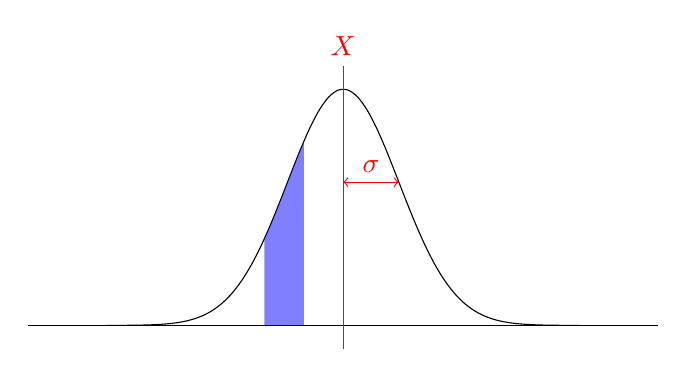
\begin{tikzpicture}[yscale=3]
      \draw (-4, 0) -- (4, 0);
      \draw plot[domain=-3:3,samples=50,smooth] (\x, {exp(-(\x*\x))});
      \fill[blue, opacity=.5] (-1, 0) -- plot[domain=-1:-.5,samples=50,smooth] (\x, {exp(-(\x*\x))}) -- (-.5, 0);
      \draw[red] (0, 1.1) node[above] {$X$} -- (0, -.1);
      \draw[<->,red] (0, 0.6065) -- node[above] {$\sigma$} (0.707, 0.6065);
    \end{tikzpicture}
  \end{center}
  \begin{equation*}
    G_{X,\sigma}(x) = \frac{1}{\sigma\sqrt{2\pi}}\,e^{-(x - X)^2 / 2\sigma^2}
  \end{equation*}
\end{frame}


\section*{Samenvatting}

\begin{frame}{Samenvatting}

  % Keep the summary *very short*.
  \begin{itemize}
  \item
    The \alert{first main message} of your talk in one or two lines.
  \item
    The \alert{second main message} of your talk in one or two lines.
  \item
    Perhaps a \alert{third message}, but not more than that.
  \end{itemize}

  % The following outlook is optional.
  \vskip0pt plus.5fill
  \begin{itemize}
  \item
    Outlook
    \begin{itemize}
    \item
      Something you haven't solved.
    \item
      Something else you haven't solved.
    \end{itemize}
  \end{itemize}
\end{frame}


\end{document}
